\documentclass[11pt,a4paper]{article}
\usepackage[margin=2.2cm]{geometry}
\usepackage{amsmath,amssymb}
\usepackage{graphicx}
\usepackage{booktabs}
\usepackage{enumitem}
\usepackage{hyperref}
\usepackage{xcolor}
\usepackage{caption}
\hypersetup{colorlinks=true,linkcolor=blue!60!black,citecolor=blue!60!black,urlcolor=blue!60!black}
\setlist{nosep,leftmargin=*}
\graphicspath{{figures/}}

\title{NeuroAI Take-Home Assignment 4\\[2pt]
\large Spiking neural networks: a neuromorphic vision front-end (design) and a Brian2 SNN on Poisson-encoded MNIST (implementation)}
\author{Anuj Tiwari \\ \texttt{anuj.tiwari@iitgn.ac.in}}
\date{\today}

\begin{document}
\maketitle

\noindent\textbf{Deliverables.} Question~1 is answered in Section~\ref{sec:q1}. Question~2 (Brian2 implementation, experiments and one main methodological tweak plus two further explorations) is reported in Section~\ref{sec:q2}; the full code, plots and analysis are in the accompanying Jupyter notebook \texttt{snn\_mnist\_experiments.ipynb} (the model code is also provided as \texttt{snn\_mnist.py}).

%=====================================================================
\section{Question 1 --- Designing an always-on neuromorphic vision front-end}
\label{sec:q1}

\paragraph{Setting.} An energy-constrained, always-on camera must detect a small set of visual events (\emph{person present}, \emph{no person}, \emph{motion only}) and must never transmit raw frames, only event-like / feature information. The design below is organised around three ideas: (i) keep the sensor-side representation \emph{sparse} (spikes only when something changes or is salient), (ii) make the network \emph{adaptive} (homeostasis and adaptation absorb slow changes in the scene so that they do not cost spikes), and (iii) keep learning \emph{local and bounded} after deployment.

%---------------------------------------------------------------------
\subsection{Encoding choice (10 marks)}

\subsubsection*{(a) Rate-based Poisson encoding}
\textbf{How it is computed.} Each pixel intensity $x_i\in[0,1]$ is mapped to a firing rate $r_i = x_i\,r_{\max}$ (e.g.\ $r_{\max}=100$~Hz). During the encoding window $T_{\mathrm{enc}}$ the pixel emits an inhomogeneous Poisson spike train: at every simulation step of length $\Delta t$ a spike is drawn with probability $r_i\Delta t$. The information is carried by the \emph{number} of spikes, $n_i\sim\mathrm{Poisson}(r_iT_{\mathrm{enc}})$; a downstream neuron or read-out decodes it by counting or low-pass filtering.

\textbf{Energy.} Poor. The number of spikes grows linearly with intensity and with the window: a $28\times28$ digit already produces $\approx 10^3$ input spikes per 100~ms (measured in Section~\ref{sec:q2}); a $128\times128$ camera frame at $r_{\max}=100$~Hz produces up to $1.6\times10^6$ spikes/s, i.e.\ bright static backgrounds are paid for continuously even when nothing happens.

\textbf{Latency of decision.} Slow. Because the count is Poisson, its signal-to-noise ratio is $\sqrt{r_iT}$, so a reliable decision needs a long window. In our MNIST experiment accuracy rises from $\approx$50\% with a 20~ms window to its plateau only after 70--100~ms (Fig.~\ref{fig:baseline_diag}). Latency and accuracy trade off directly.

\textbf{Robustness to noise.} Good. Counting averages out timing jitter, random spike loss and additive sensor noise; the code is insensitive to the exact arrival times and to the neuron model of the decoder; degradation under noise is graceful.

\subsubsection*{(b) Latency / temporal (time-to-first-spike) encoding}
\textbf{How it is computed.} Each pixel emits \emph{at most one} spike whose timing is a decreasing function of intensity, e.g.\ linear $t_i = T_{\max}(1-x_i)$ or logarithmic $t_i=\tau\ln(x_{\max}/x_i)$ (the latter is what a leaky integrator charged by a current $\propto x_i$ naturally produces); pixels below an intensity threshold never spike. Brighter pixels fire earlier, so the information is in the \emph{order} and relative times of the first spikes (rank-order code). It is decoded by neurons with short membrane time constants or synaptic delays that are sensitive to coincidence/order, or by a read-out with a decaying temporal kernel so that early spikes get the largest weight.

\textbf{Energy.} Excellent: $\le 1$ spike per pixel per frame, independent of intensity, and in practice far fewer because dark/unchanged pixels are below threshold. For the camera above this is $\le 1.6\times10^4$ spikes per frame instead of $10^6$/s.

\textbf{Latency of decision.} Fast. The most salient (brightest / highest-contrast) pixels arrive first, so a decision can be made after the first few percent of spikes have arrived (``first $k$ spikes'' decoding), typically within a few milliseconds of the frame onset, without waiting for the end of the window.

\textbf{Robustness to noise.} Weaker. (i) A single spurious early spike (hot pixel, sensor noise) is placed at the front of the order and corrupts the code; (ii) timing jitter directly perturbs the code, so it needs precise synchronisation to a frame-onset reference; (iii) a global illumination change shifts \emph{all} latencies, so the code must be made relative (rank order / normalised to the first spike); (iv) dim pixels contribute no information until late in the window.

\subsubsection*{Choice for the rapid detection of a rare event}
I would choose the \textbf{latency (temporal) encoding}, applied to \emph{temporal contrast} (pixel changes, as in a DVS event camera) rather than to absolute intensity. The reasons follow directly from the comparison above: (1)~a rare event means the sensor is idle most of the time; with latency coding of changes, idle time costs almost no spikes, whereas rate coding keeps paying for the static scene; (2)~the decision latency is bounded by the arrival of the first, most salient spikes rather than by the window length needed to beat Poisson counting noise; (3)~the lower noise robustness can be bought back cheaply---an intensity/contrast threshold on the encoder removes most spurious early spikes, decoding the \emph{rank} rather than absolute times removes sensitivity to illumination, and a short confirmation stage that accumulates a few spikes (a hybrid ``first-spikes decision, count-based confirmation'') controls the false-alarm rate. Rate coding would be preferred only if the sensor noise were so high that counting over a long window is unavoidable, which is exactly the regime where an always-on, energy-constrained detector cannot operate anyway.

%---------------------------------------------------------------------
\subsection{Network architecture (10 marks)}

\textbf{Overview (four stages).}
\begin{enumerate}
\item \textbf{Input / event layer} (no neurons, $2\times 64\times64 = 8192$ channels). The sensor output (DVS events, or frame differences from a conventional sensor) is downsampled to $64\times64$ with separate ON and OFF polarity channels; each channel emits a latency-coded spike when the local contrast change exceeds a threshold. \emph{Role:} sparse, change-driven, illumination-invariant representation; no raw frame ever leaves the sensor.
\item \textbf{Feature layer} ($8$ feature maps $\times 32\times32 = 8192$ LIF neurons). Each neuron has a local $5\times5$ receptive field (stride 2) over both polarity channels; neurons within a map share no weights on neuromorphic hardware, but are initialised identically and learn oriented edge / motion-direction detectors by STDP (Section~\ref{sec:plasticity}). Lateral inhibition (soft winner-take-all among the 8 neurons that look at the same location) decorrelates the maps and keeps activity sparse. \emph{Neuron type:} plain LIF with a \emph{short} membrane time constant ($\tau_m\approx 5$--10~ms) and a 2~ms refractory period, so that they act as coincidence detectors on the latency code (only near-simultaneous early spikes within the receptive field drive them). Our MNIST experiment shows why short $\tau_m$ matters here: a long $\tau_m$ smooths spike timing, raises firing rates and the first-spike latency.
\item \textbf{Integration layer} ($500$ adaptive LIF neurons, recurrent). Receives the feature layer through \emph{sparse random} excitatory projections ($p_{\mathrm{conn}}\approx 0.05$; each integration neuron sees $\approx 400$ feature neurons) and has sparse random recurrent connectivity ($p\approx0.1$) with 80\% excitatory / 20\% inhibitory neurons, i.e.\ a small balanced reservoir. \emph{Neuron type:} adaptive LIF (ALIF): the threshold increases by a fixed amount after every spike and decays back with $\tau_a\approx 300$~ms. Adaptation gives the layer (i) a memory of the last few hundred milliseconds, which is what distinguishes ``motion only'' (transient, uncorrelated activity) from ``person present'' (sustained, spatially structured activity), and (ii) automatic suppression of anything static or repetitive---a flickering light or a swaying tree stops driving the network after a few cycles. Sparse random connectivity is chosen deliberately: in Section~\ref{sec:conn} we show that sparse random projections produce far more diverse (less correlated) features than dense ones at the same mean drive and the same number of spikes, so the read-out sees a richer code.
\item \textbf{Read-out} (3 LIF output neurons, one per event class). A \emph{spiking} linear read-out: each output neuron integrates the low-pass-filtered spike counts of the integration layer (exponential kernel, $\tau\approx 100$~ms) through weights trained offline as a linear classifier on spike-count features (exactly the scheme implemented in Question~2, but with the trained weights loaded into three integrate-and-fire units). Mutual inhibition between the three units implements winner-take-all; the first output neuron to fire \emph{is} the transmitted event (class id + timestamp), so the radio is only used when a decision is made. A count-based read-out is preferred over a purely temporal one because it is robust to the Poisson-like variability of the integration layer, and the low-pass kernel lets the \emph{latency-to-decision} be tuned by a single parameter.
\end{enumerate}
The whole front-end has $\approx 1.7\times10^4$ neurons and $\approx 0.6\times10^6$ synapses, which fits on a single core group of a neuromorphic chip (e.g.\ one Loihi chip or a fraction of SpiNNaker board), and the only output is $\le$ a few events per second.

%---------------------------------------------------------------------
\subsection{Plasticity and adaptation (10 marks)}
\label{sec:plasticity}

\textbf{Which rule where, and why.}
\begin{itemize}
\item \textbf{Input $\to$ feature layer: unsupervised STDP with synaptic scaling.} Pair-based (or triplet) STDP with an exponential window ($A_+ > A_-$, $\tau_\pm\approx 20$~ms) learns the spatio-temporal correlations of the event stream, i.e.\ oriented edges and motion directions, from \emph{unlabelled} data; weight normalisation (the incoming weights of each neuron sum to a constant) and lateral inhibition prevent run-away potentiation and force different maps to learn different features (the Diehl--Cook recipe). STDP is the natural choice here because the useful features are statistics of the input, not of the labels, and because it is local and cheap on neuromorphic hardware.
\item \textbf{Feature $\to$ integration layer and recurrent synapses: fixed random weights + short-term depression + intrinsic homeostasis.} The projection is kept random (reservoir computing) so that no gradient has to be propagated into a recurrent spiking network. Short-term synaptic depression (Tsodyks--Markram) on the feed-forward synapses makes the integration layer respond to \emph{onsets} and novelty, which is what ``motion only'' needs. Each integration neuron has an intrinsic homeostatic rule (as implemented in Section~\ref{sec:homeo}): its threshold $\theta_i$ integrates $(r_i - r_{\mathrm{target}})$ with its own low-passed rate $r_i$, so that the layer stays in the dynamic range where the read-out is informative regardless of the ambient activity level. This also fixes the energy budget of the layer (spikes/s $\approx N\,r_{\mathrm{target}}$).
\item \textbf{Integration $\to$ read-out: supervised, reward-modulated plasticity.} The read-out weights are trained offline from labelled spike-count features (linear classifier) and refined online with reward-modulated STDP (R-STDP): an eligibility trace is formed by pre/post coincidences and consolidated only when a (sparse) reward/teacher signal arrives, e.g.\ a user confirmation or a verdict from a cloud model on the rare occasions when a snippet is uploaded. This is the only place where labels are needed, and it is a single, shallow layer, so a three-factor rule is sufficient.
\end{itemize}

\textbf{Adapting to new environments without catastrophic forgetting.}
\begin{enumerate}
\item \emph{Separate fast and slow variables.} After factory training the STDP feature layer is frozen (or its learning rate reduced by $10^{2}$--$10^{3}$ and its weights bounded); the variables that keep adapting in the field are the \emph{homeostatic thresholds} and \emph{adaptation currents}, which are not synaptic weights at all. A new room, a different illumination or a different camera angle changes the activity statistics, and the homeostatic thresholds absorb that within tens of seconds (Section~\ref{sec:homeo}, Fig.~\ref{fig:homeo}) without touching what the network has learned.
\item \emph{Protect important synapses (metaplasticity / consolidation).} For the synapses that do remain plastic, each weight carries an importance estimate (e.g.\ the magnitude of its eligibility trace integrated over the training history, as in EWC/synaptic intelligence, or a Benna--Fusi cascade of slow variables). The effective learning rate is scaled by $1/(1+\Omega_{ij})$, so synapses that were important for the old environment change slowly, while unused synapses are free to learn the new one.
\item \emph{Environment-specific read-out heads.} The integration layer is shared; the read-out is cheap (3 neurons $\times$ 500 weights), so a new head can be allocated per environment / context (selected by an index or by a small context-detection neuron). Learning a new head cannot overwrite an old one.
\item \emph{Sparse replay.} A tiny buffer of compressed \emph{feature-layer} spike patterns (not frames; typically a few hundred patterns of a few hundred bytes) is stored on-chip and replayed, interleaved with the new data, whenever the read-out is updated. Interleaving is the simplest and most effective protection against forgetting in a single linear layer.
\item \emph{Normalisation as a safety net.} Synaptic scaling keeps the total incoming weight of every neuron constant, so new learning redistributes weight rather than adding it; combined with the bounded weights this guarantees that adaptation can never silence or saturate the network.
\end{enumerate}

%---------------------------------------------------------------------
\subsection{Evaluation and metrics (10 marks)}

\textbf{Data.} Three complementary sources, in increasing order of realism.
\begin{itemize}
\item \emph{Synthetic event streams.} Person silhouettes / moving objects from a 3D renderer composited onto static and dynamically changing backgrounds, converted to events with a DVS simulator (e.g.\ v2e/ESIM), with controlled illumination, noise level (hot pixels, background activity events) and event onset time. This gives exact ground truth for \emph{latency} and lets us sweep noise systematically.
\item \emph{Public neuromorphic datasets} for sanity checks of the pipeline: N-MNIST / DVS-Gesture (basic recognition in the event domain) and pedestrian/person DVS datasets (e.g.\ DVS pedestrian detection, PAFBenchmark) for the actual task.
\item \emph{Own recordings with the target sensor.} Protocol: a DAVIS (events + frames) or a frame camera with on-sensor frame differencing, mounted in $\ge 5$ locations (indoor/outdoor), day and night, $\ge 10$ sessions each; the three classes are labelled from the synchronised frames by annotators; crucially the set must contain \emph{many hours of ``no person''} footage (vehicles, animals, lighting changes, rain) because the false-alarm rate is the metric that dominates the energy of an always-on device. Splits are by location so that generalisation to unseen environments is measured.
\end{itemize}

\textbf{Metrics.}
\begin{itemize}
\item \emph{Task performance:} accuracy and macro-F1 over the three classes, plus the person-present precision/recall curve; \emph{false alarms per hour} on the ``no person'' footage and miss rate at a fixed false-alarm budget (e.g.\ $\le 1$/h).
\item \emph{Latency to detection:} time from the labelled event onset to the first read-out spike; report the median and the 95th percentile, and the full accuracy-versus-decision-window curve (as in Fig.~\ref{fig:baseline_diag}).
\item \emph{Energy proxies:} average firing rate per layer (Hz/neuron), total spikes/s, synaptic operations/s (spikes $\times$ fan-out), and the transmitted bit rate (events/s $\times$ bits/event) compared with the raw-frame rate; converted to Joules with a per-SOP cost of the target chip (e.g.\ $\approx 20$~pJ/SOP on Loihi). We report the full curve of accuracy versus spikes/image because, as the MNIST experiments show, accuracy and spikes can be traded against each other through $\tau_m$, weights and thresholds.
\item \emph{Robustness:} the metrics above as a function of injected noise events/s, illumination change and spike-drop probability.
\end{itemize}

\textbf{Ablations and expectations.}
\begin{enumerate}
\item \emph{Disable homeostasis / adaptation.} Expect activity to drift with illumination and scene statistics: some neurons saturate, others go silent, accuracy drops in environments that differ from the training one and spike rate (energy) becomes uncontrolled; the ALIF adaptation ablation should specifically raise false alarms from flicker and repetitive motion.
\item \emph{Change the encoding} (latency $\to$ rate, or absolute intensity instead of temporal contrast). Expect an order of magnitude more spikes, a longer latency to detection, but somewhat better robustness to hot-pixel noise.
\item \emph{Membrane time constant of the feature layer} ($\tau_m = 5, 20, 50$~ms). Expect long $\tau_m$ to blur the latency code, raise rates and lengthen the first-spike latency (observed in Section~\ref{sec:tau}); short $\tau_m$ to be more selective but more sensitive to spike loss.
\item \emph{Dense vs.\ sparse feature $\to$ integration projection.} Expect dense random projections to produce highly redundant features (every neuron mostly measures total activity) and sparse ones to be more diverse and more accurate at equal spike count (observed in Section~\ref{sec:conn}).
\item \emph{Remove lateral inhibition / STDP in the feature layer (random fixed filters).} Expect redundant maps and a lower accuracy at equal size; the random-filter result gives the floor that learning has to beat.
\item \emph{Read-out window.} Sweeping the kernel time constant maps the latency--accuracy--false-alarm trade-off and selects the operating point.
\end{enumerate}

%=====================================================================
\section{Question 2 --- Feed-forward SNN on Poisson-encoded MNIST (Brian2)}
\label{sec:q2}

\subsection{Model and implementation}

\textbf{Encoding.} Each $28\times28$ image is flattened to $N_{\mathrm{in}}=784$ Poisson sources with rate $r_i = x_i\cdot 100$~Hz ($x_i\in[0,1]$) for an encoding interval $T_{\mathrm{enc}}=100$~ms (on average $\approx 10^3$ input spikes per image).

\textbf{Hidden layer.} $N_h = 300$ leaky integrate-and-fire neurons,
\[
\tau_m \frac{dv}{dt} = V_{\mathrm{rest}} - v,\qquad v \leftarrow v + w_{ij}\ \text{on an input spike},\qquad
v>V_{\mathrm{th}}\Rightarrow \text{spike},\ v\leftarrow V_{\mathrm{reset}},
\]
with $\tau_m = 20$~ms, $V_{\mathrm{rest}}=V_{\mathrm{reset}}=-70$~mV, $V_{\mathrm{th}}=-50$~mV and an absolute refractory period of 2~ms (Euler integration, $\Delta t=0.1$~ms). Synapses are instantaneous current-based EPSPs with excitatory weights $w_{ij} = w_{\mathrm{scale}}\,\tilde w_{ij}$, $\tilde w_{ij}\sim\mathcal N(0.5,0.1)$ clipped to be non-negative, masked by a Bernoulli connectivity mask with probability $p_{\mathrm{conn}}$. The baseline uses \emph{fractional} connectivity $p_{\mathrm{conn}}=0.2$ (fan-in $\approx 157$) and $w_{\mathrm{scale}}=1.25$~mV, chosen so that the mean hidden rate is $\approx 25$~Hz. The membrane potential is reset at every image boundary, so images are independent. All weights are frozen (no learning in the SNN).

\textbf{Read-out.} For each image the spike count of every hidden neuron over $T_{\mathrm{enc}}$ is the feature vector ($\mathbb R^{300}$). An \texttt{sklearn} logistic-regression classifier (standardised features, L2 regularisation $C=0.1$) is trained offline on the first 5\,000 MNIST training images and evaluated on the first 1\,000 test images. For reference, the same classifier trained on the raw pixels of the same 5\,000 images is reported.

\textbf{Efficient simulation.} With the pure-\texttt{numpy} Brian2 back-end, calling \texttt{run()} once per image is prohibitively slow. Instead, $B=25$ independent copies of the network are built in one \texttt{Network} (block-diagonal synapse matrix), the Poisson rates of the whole data set are stored in a 2-D \texttt{TimedArray} with $dt = T_{\mathrm{enc}}$, and a single \texttt{run()} streams all images through the network; a \texttt{run\_regularly} operation resets $v$ at every image boundary. Hidden spikes are binned per (image, neuron, 10-ms bin), which costs nothing extra and allows the accuracy-versus-decision-window analysis. 6\,000 images are simulated in about 2.5~minutes on a laptop.

\subsection{Baseline results}
\label{sec:baseline}

\begin{figure}[h]
\centering
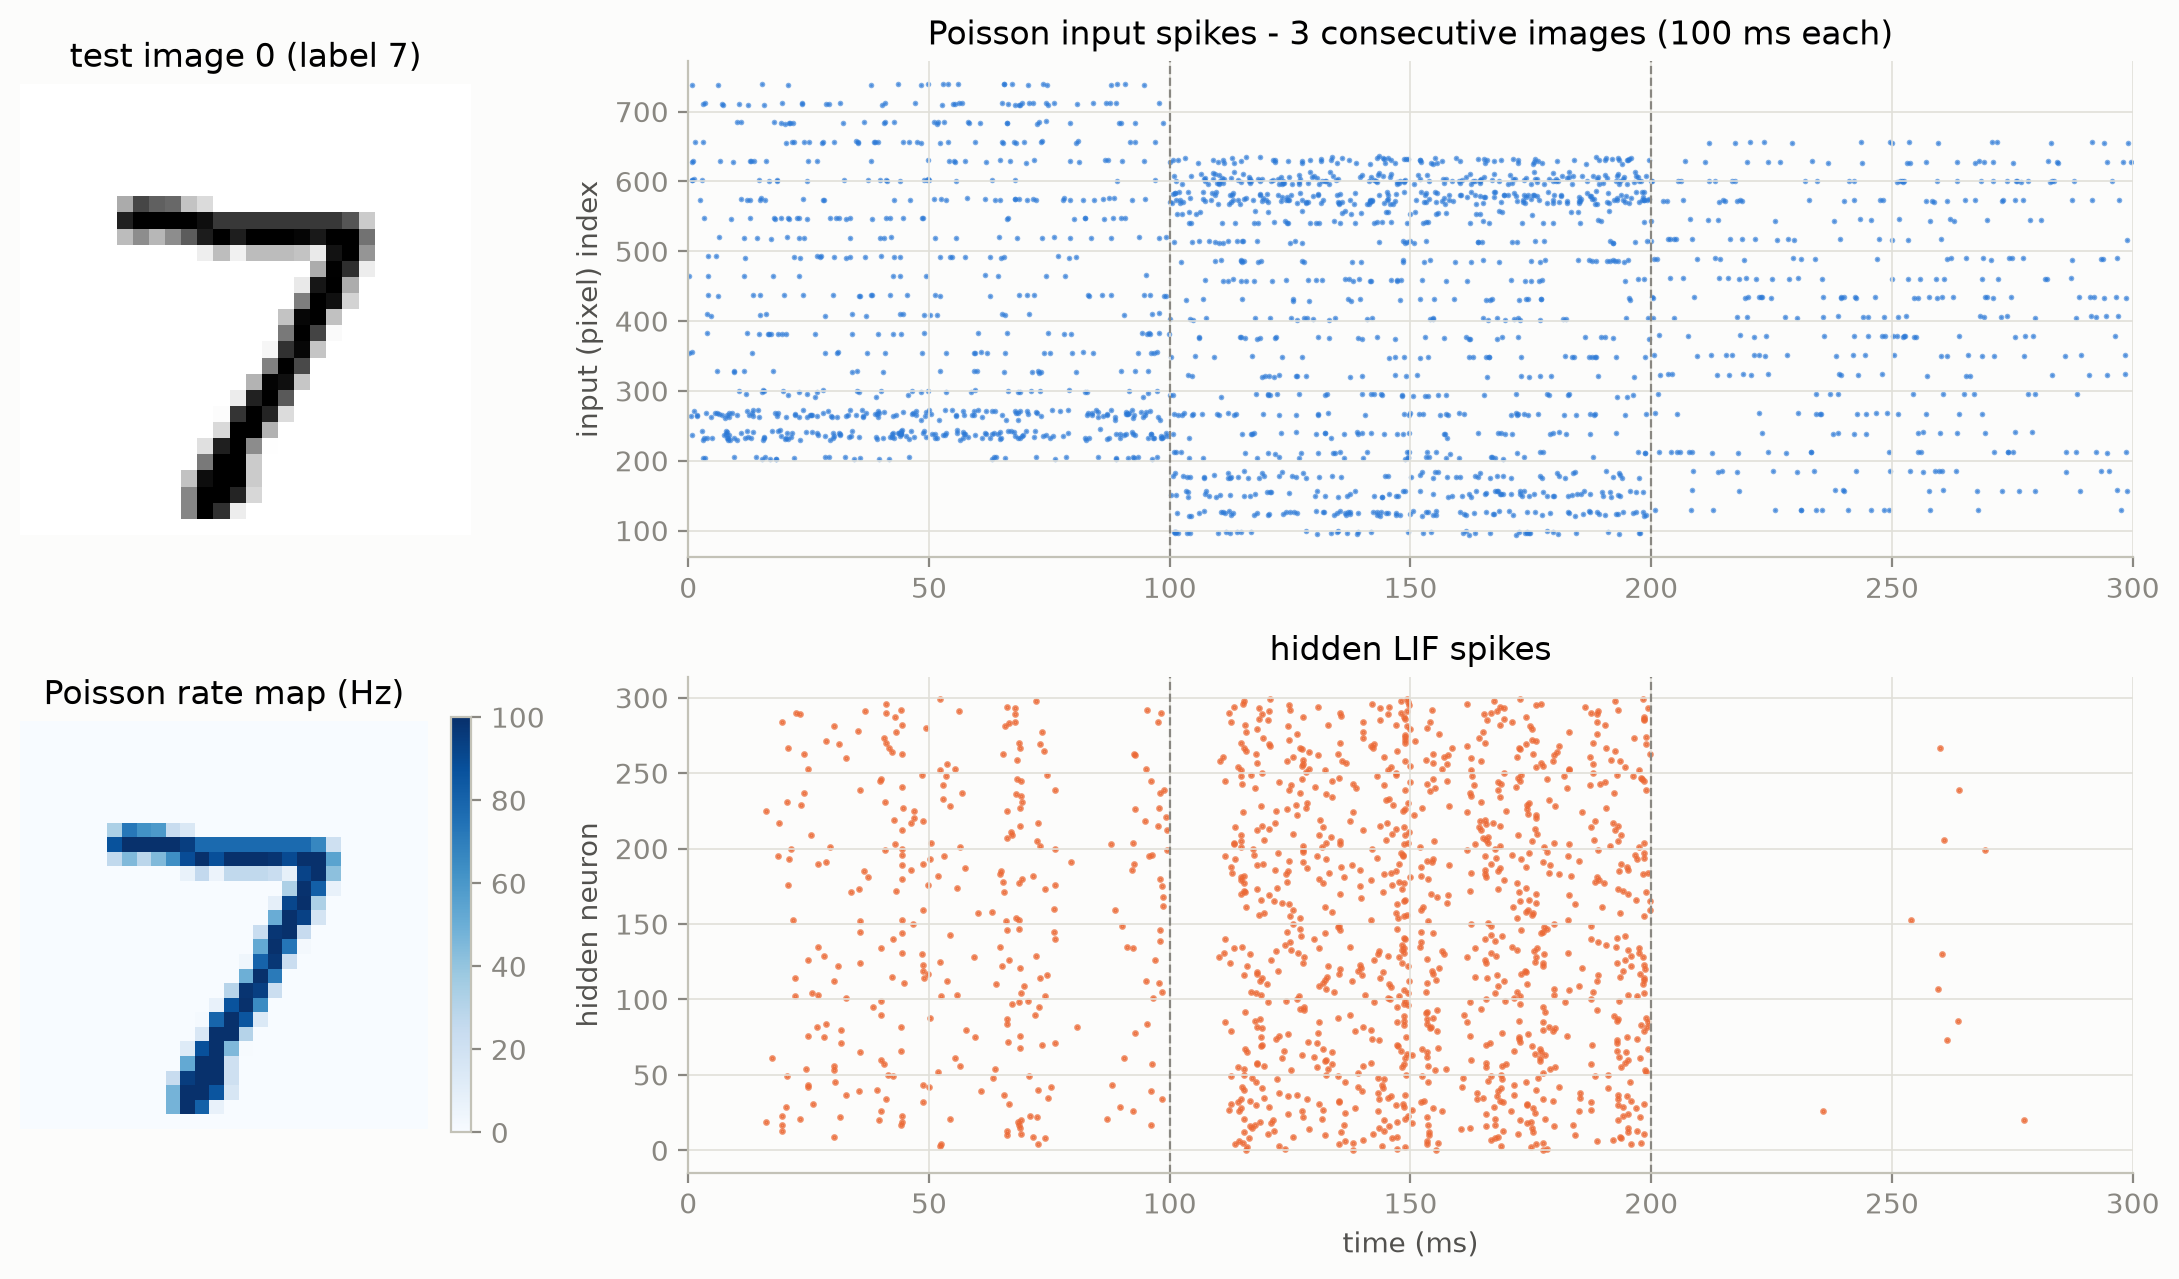
\includegraphics[width=0.95\textwidth]{fig_baseline_rasters.png}
\caption{Baseline network on three consecutive test images. Left: the image and its Poisson rate map. Right: Poisson input spikes (top) and hidden-layer spikes (bottom). Note that the thin digit in the third slot (a ``1'') produces far fewer input spikes and almost no hidden spikes: with purely excitatory, non-normalised weights the drive of every hidden neuron scales with the total ``ink'' of the image.}
\label{fig:baseline_rasters}
\end{figure}

\begin{figure}[h]
\centering
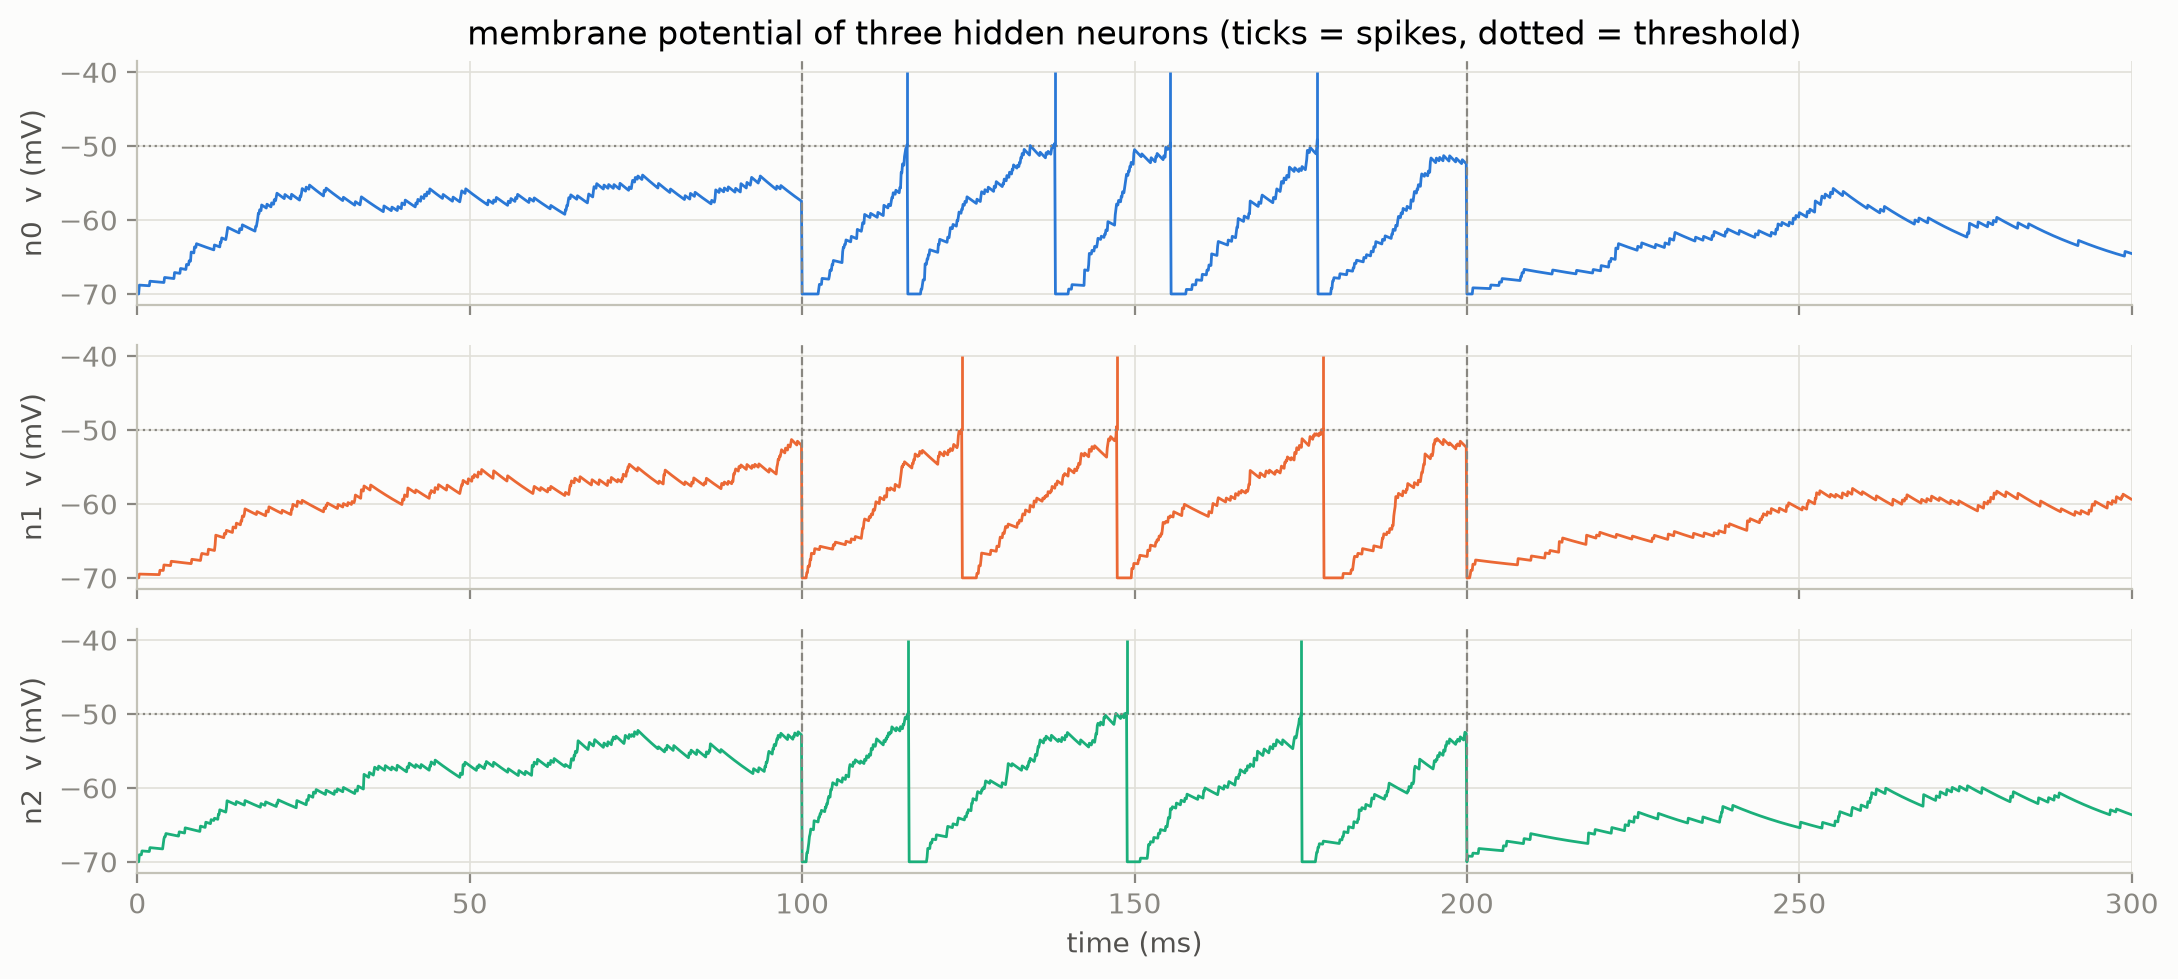
\includegraphics[width=0.95\textwidth]{fig_baseline_vtraces.png}
\caption{Membrane potential of three hidden neurons during the same three images (dotted line: threshold; ticks: spikes). Resets at the image boundaries are visible as drops to $V_{\mathrm{rest}}$.}
\label{fig:baseline_vtraces}
\end{figure}

\begin{figure}[h]
\centering
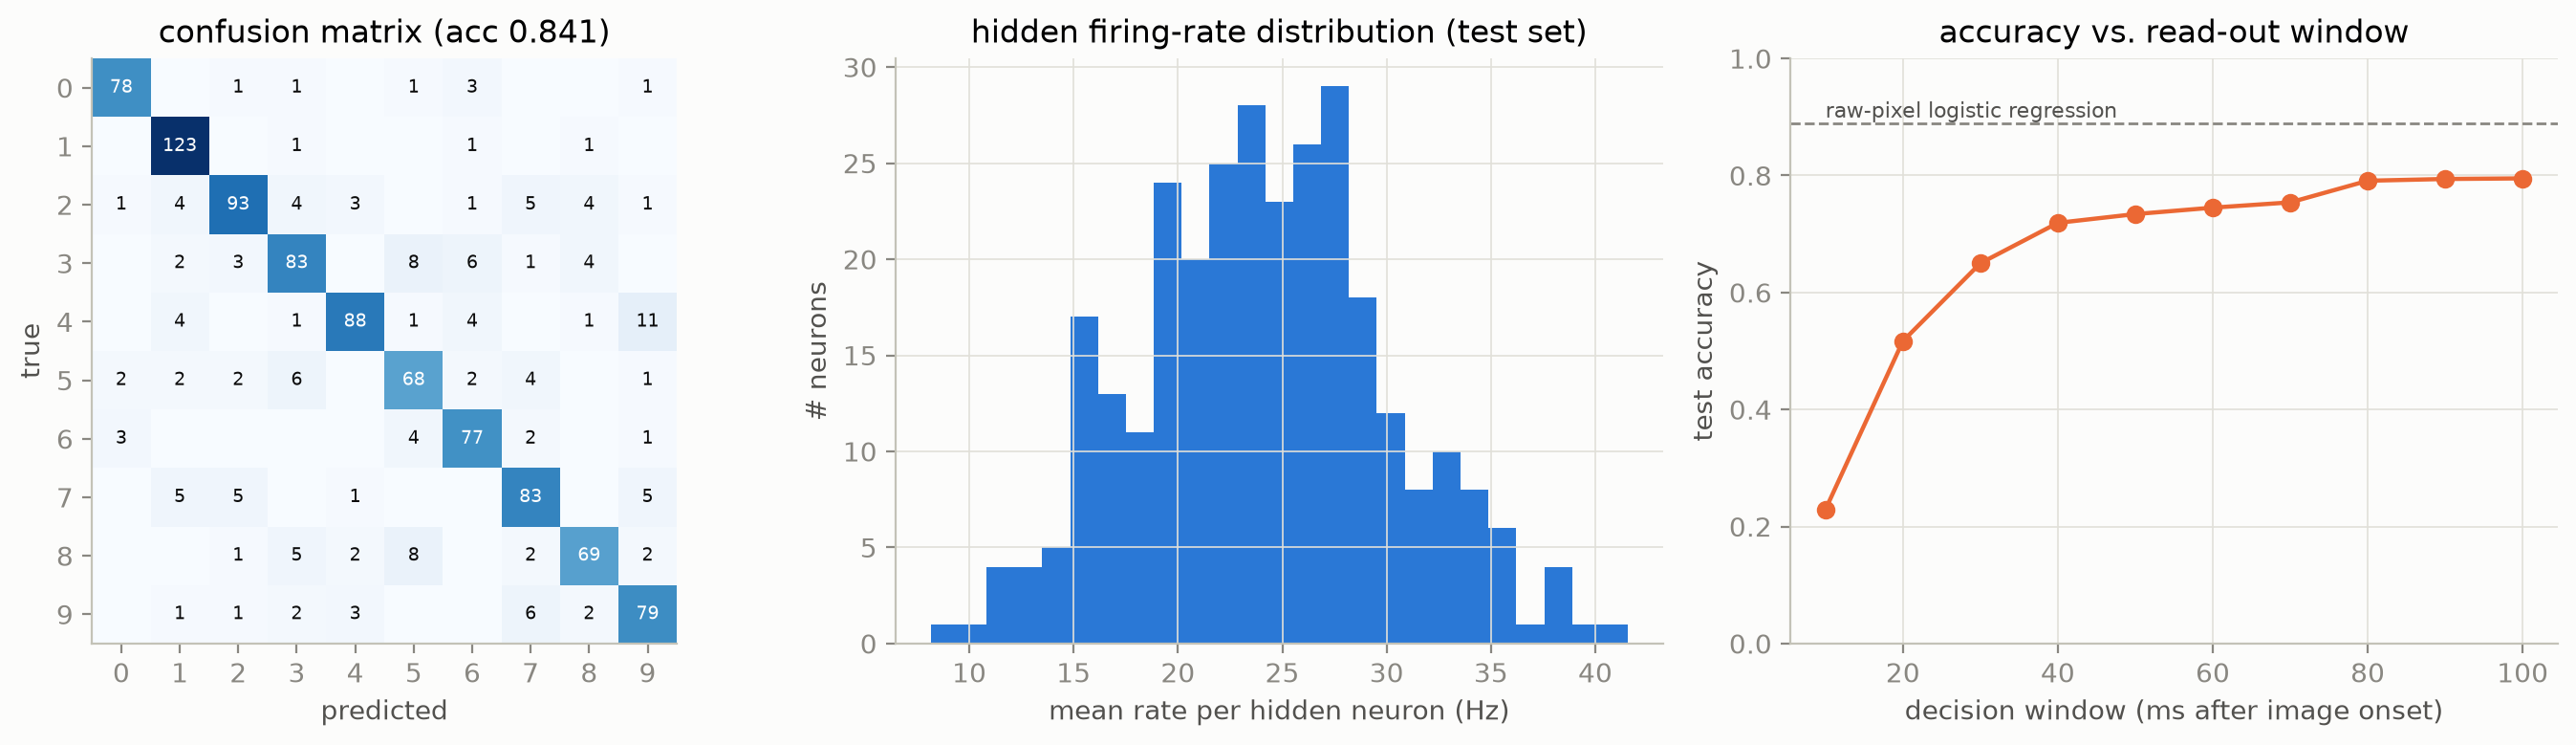
\includegraphics[width=\textwidth]{fig_baseline_diag.png}
\caption{Baseline diagnostics. Left: confusion matrix on the 1\,000 test images. Middle: distribution of the mean firing rate of the 300 hidden neurons. Right: test accuracy when the read-out only sees the spikes emitted in the first $t$ ms after image onset (latency-to-decision curve); the dashed line is the raw-pixel logistic regression.}
\label{fig:baseline_diag}
\end{figure}

\begin{table}[h]
\centering
\caption{Baseline performance (5\,000 training / 1\,000 test images).}
\label{tab:baseline}
\begin{tabular}{lcccc}
\toprule
Model & Test accuracy & Macro-F1 & Mean hidden rate (Hz) & Hidden spikes / image\\
\midrule
SNN spike counts + logistic regression & BASE\_ACC & BASE\_F1 & BASE\_RATE & BASE\_SPK\\
Raw pixels + logistic regression (reference) & PIX\_ACC & -- & -- & --\\
\bottomrule
\end{tabular}
\end{table}

BASELINE\_ANALYSIS

\subsection{Tweak 1 (main): systematically varying the membrane time constant $\tau_m$}
\label{sec:tau}

$\tau_m$ is swept over $\{5, 10, 20, 50\}$~ms in two regimes. (i) \emph{Fixed weights}: everything else is kept at the baseline value. Because the mean depolarisation of an LIF neuron under a Poisson barrage is $\bar v - V_{\mathrm{rest}} \approx \tau_m\sum_i w_i r_i$, changing $\tau_m$ also changes the mean drive, so firing rates change dramatically. (ii) \emph{Drive-matched weights}: $w_{\mathrm{scale}} \propto 1/\tau_m$ (i.e.\ $1.25\,\mathrm{mV}\times 20/\tau_m$), which keeps the mean depolarisation constant and isolates the effect of the integration window (temporal smoothing) from that of the mean drive. For every setting we record accuracy, F1, mean rate, spikes per image, the population PSTH, the mean latency of the first hidden spike after image onset (20 test images) and an example voltage trace.

\begin{figure}[h]
\centering
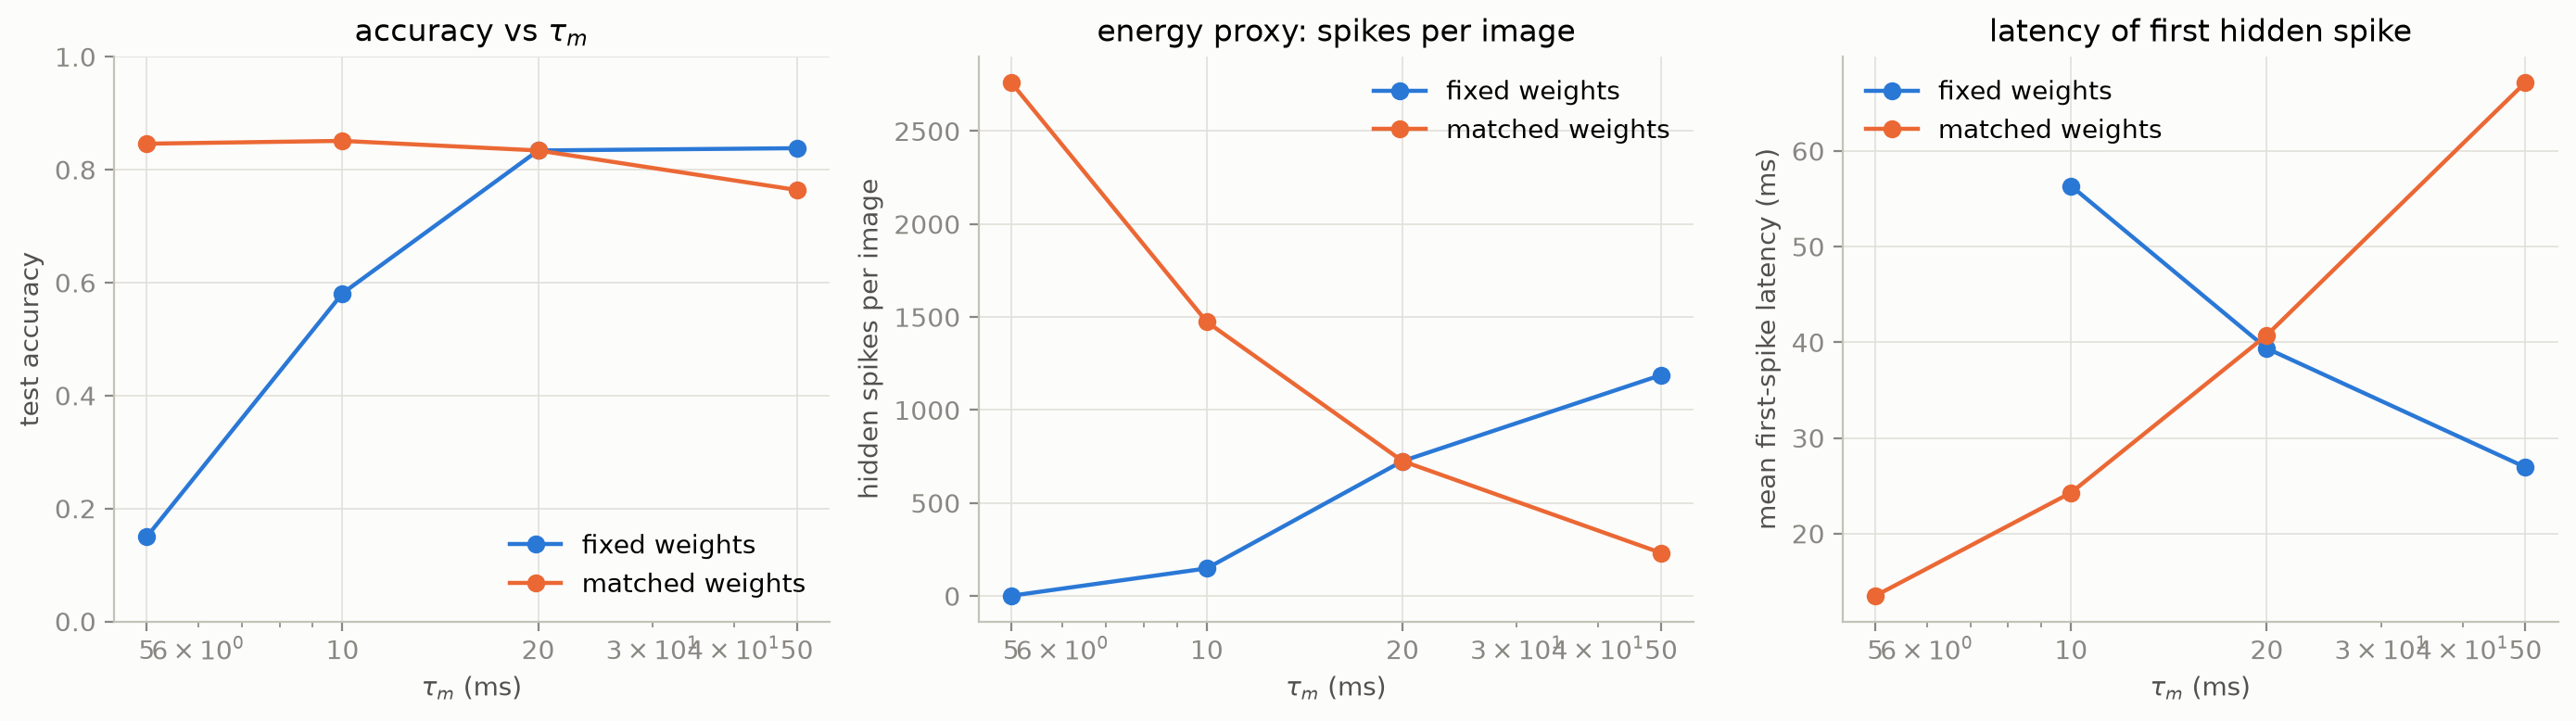
\includegraphics[width=\textwidth]{fig_tau_sweep.png}
\caption{$\tau_m$ sweep. Left: test accuracy; middle: hidden spikes per image (energy proxy); right: mean first-spike latency. Blue: fixed weights; orange: drive-matched weights ($w_{\mathrm{scale}}\propto 1/\tau_m$).}
\label{fig:tau_sweep}
\end{figure}

\begin{figure}[h]
\centering
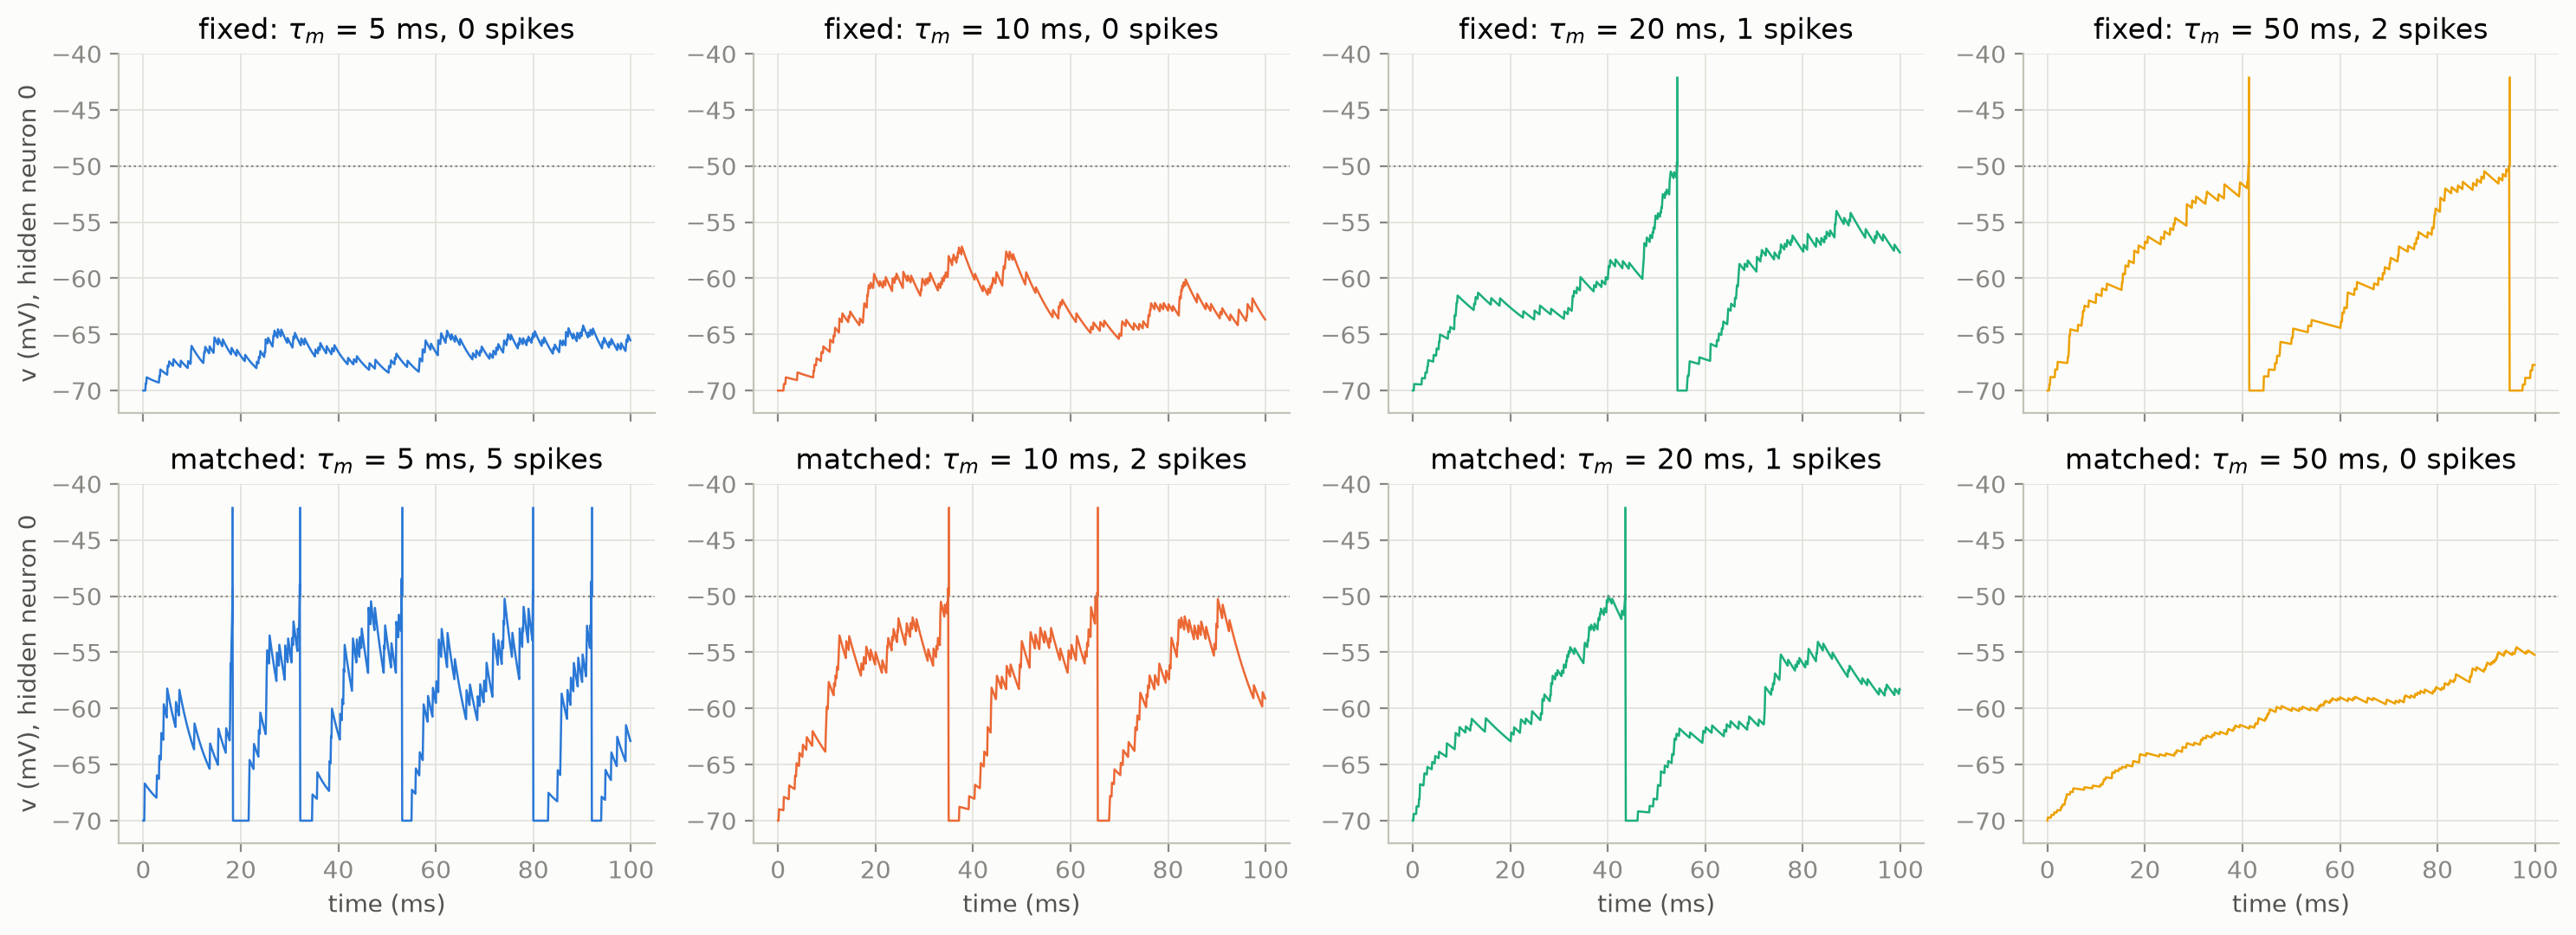
\includegraphics[width=\textwidth]{fig_tau_vtraces.png}
\caption{Example voltage traces of hidden neuron 0 for the first 100~ms of a test image at each $\tau_m$ (top: fixed weights, bottom: drive-matched weights).}
\label{fig:tau_vtraces}
\end{figure}

\begin{figure}[h]
\centering
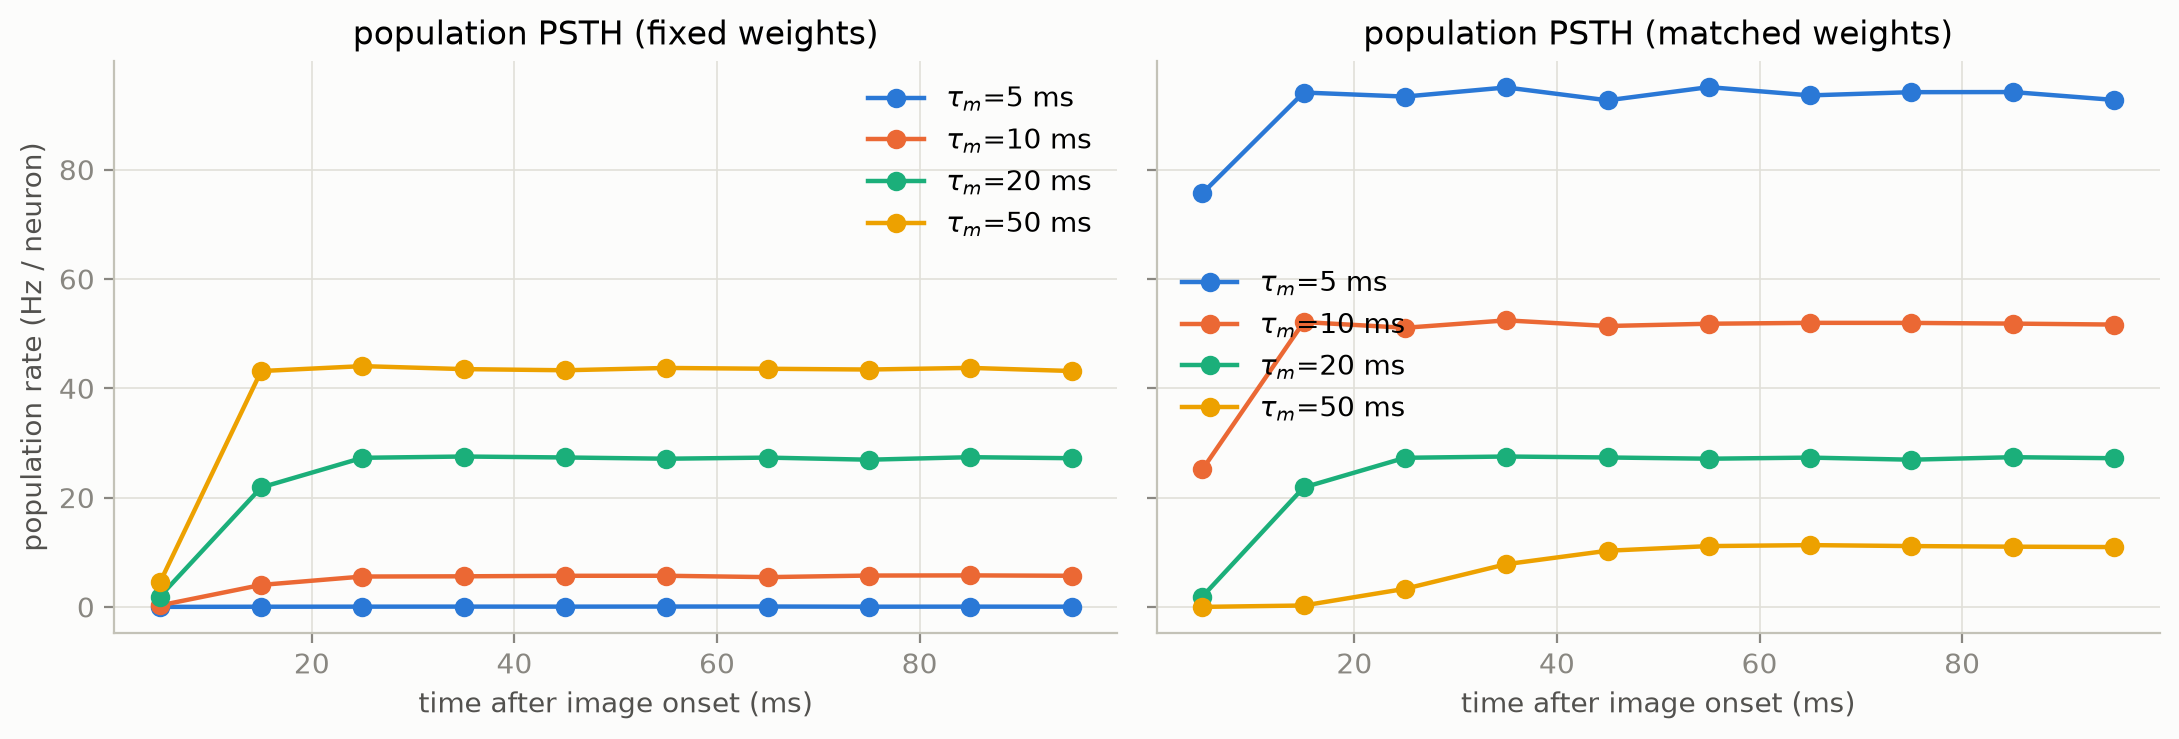
\includegraphics[width=0.9\textwidth]{fig_tau_psth.png}
\caption{Population PSTH (mean rate per hidden neuron in 10-ms bins after image onset) for each $\tau_m$.}
\label{fig:tau_psth}
\end{figure}

\begin{table}[h]
\centering
\caption{Effect of $\tau_m$ on firing, timing and classification.}
\label{tab:tau}
\begin{tabular}{llccccc}
\toprule
Regime & $\tau_m$ (ms) & Accuracy & Macro-F1 & Rate (Hz) & Spikes/image & First spike (ms)\\
\midrule
TAU\_ROWS
\bottomrule
\end{tabular}
\end{table}

TAU\_ANALYSIS

\subsection{Tweak 2: sparse connectivity}
\label{sec:conn}

The connection probability is swept over $p_{\mathrm{conn}}\in\{1.0, 0.5, 0.2, 0.1, 0.05, 0.02\}$ (1.0 = dense; 0.05 = the value suggested in the assignment) with $w_{\mathrm{scale}} = 0.25\,\mathrm{mV}/p_{\mathrm{conn}}$ so that the \emph{mean} drive per hidden neuron is identical for every $p_{\mathrm{conn}}$ (the baseline is the $p_{\mathrm{conn}}=0.2$ point). Besides accuracy and spikes we measure how redundant the hidden code is: the mean pairwise Pearson correlation between the spike counts of different hidden neurons across the test images.

\begin{figure}[h]
\centering
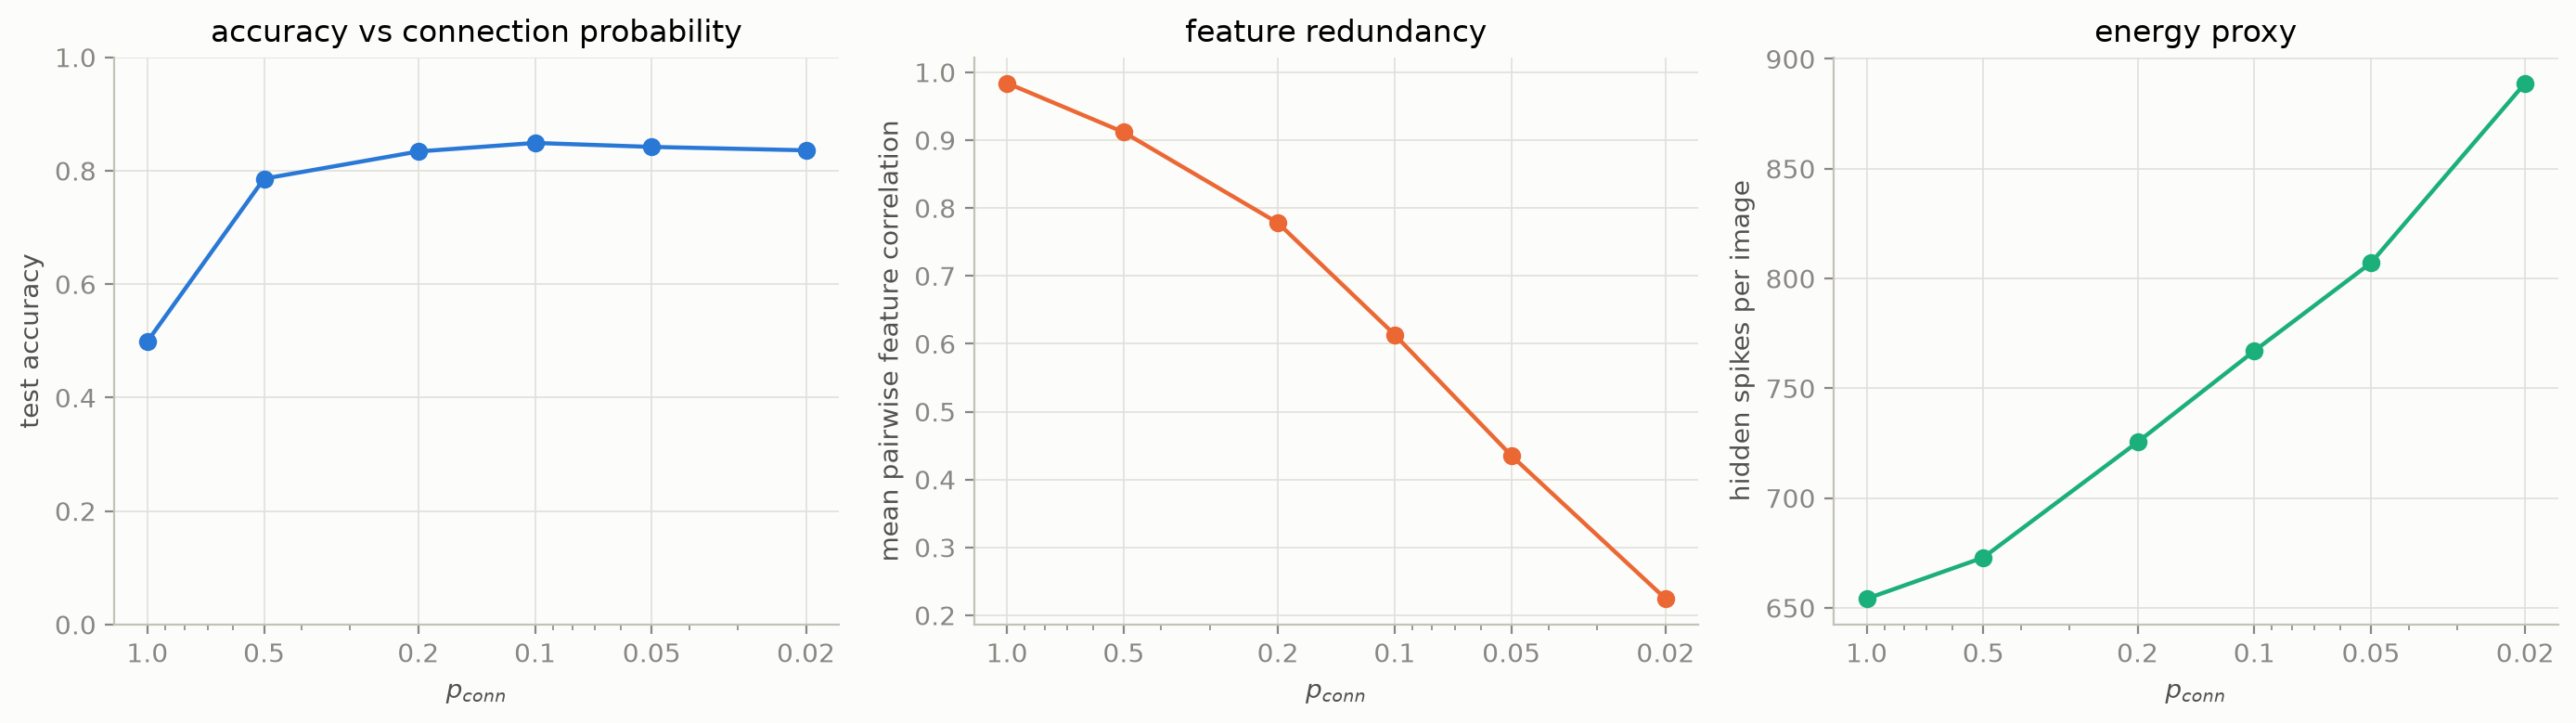
\includegraphics[width=\textwidth]{fig_conn_sweep.png}
\caption{Connectivity sweep (dense on the left, sparser to the right). Left: accuracy; middle: mean pairwise correlation of hidden features; right: hidden spikes per image.}
\label{fig:conn_sweep}
\end{figure}

\begin{figure}[h]
\centering
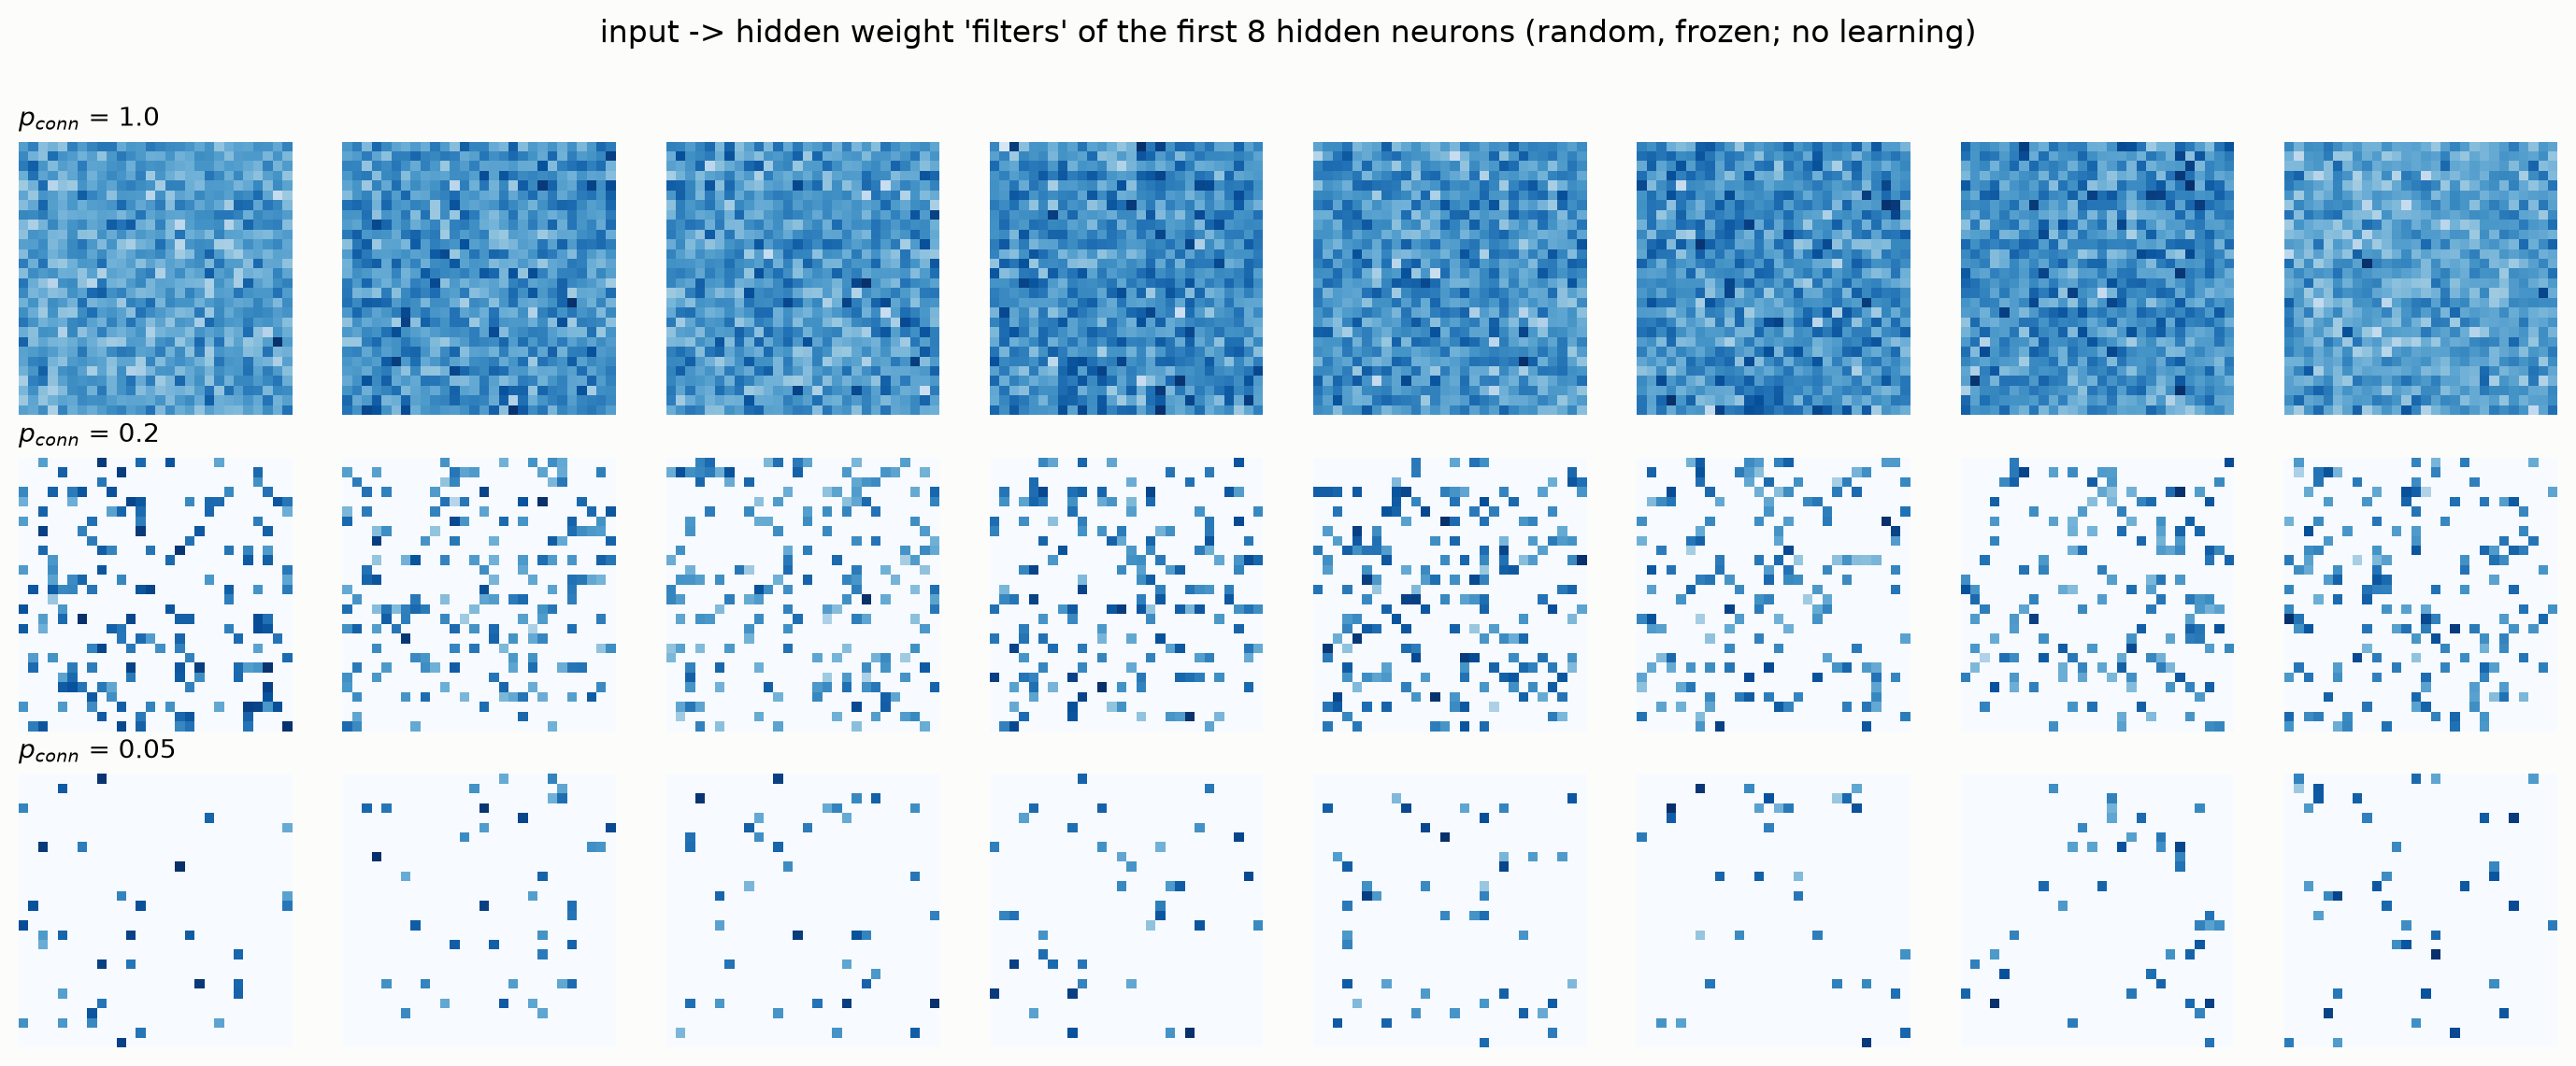
\includegraphics[width=\textwidth]{fig_conn_filters.png}
\caption{Input$\to$hidden weight ``filters'' (the 784 incoming weights of the first 8 hidden neurons reshaped to $28\times28$) for dense, $p=0.2$ and $p=0.05$ connectivity. Weights are random and frozen, so these are the initial (= final) filters.}
\label{fig:conn_filters}
\end{figure}

\begin{table}[h]
\centering
\caption{Effect of the connection probability (matched mean drive).}
\label{tab:conn}
\begin{tabular}{lccccc}
\toprule
$p_{\mathrm{conn}}$ & Fan-in & Accuracy & Macro-F1 & Spikes/image & Feature correlation\\
\midrule
CONN\_ROWS
\bottomrule
\end{tabular}
\end{table}

CONN\_ANALYSIS

\subsection{Tweak 3: homeostatic firing-rate regulation}
\label{sec:homeo}

Each hidden neuron receives an adaptive threshold $\theta_i$ and a low-pass estimate $r_i$ of its own rate,
\[
\frac{dr_i}{dt} = -\frac{r_i}{\tau_r} \;\Big(+\frac{1}{\tau_r}\ \text{at each spike}\Big),\qquad
\frac{d\theta_i}{dt} = \eta\,(r_i - r_{\mathrm{target}}),\qquad \theta_i\in[V_{\mathrm{rest}}+2\,\mathrm{mV},\,V_{\mathrm{th}}+60\,\mathrm{mV}],
\]
with $\tau_r = 0.5$~s and $\eta = 0.5$~mV. A neuron firing above its target raises its threshold and vice versa. The rule runs on a 500-image calibration stream (50~s) taken from the training set; the thresholds are then frozen and the train/test protocol of the baseline is repeated. Targets of 10~Hz and 20~Hz are tested (the baseline mean rate is $\approx 25$~Hz with a wide spread).

\begin{figure}[h]
\centering
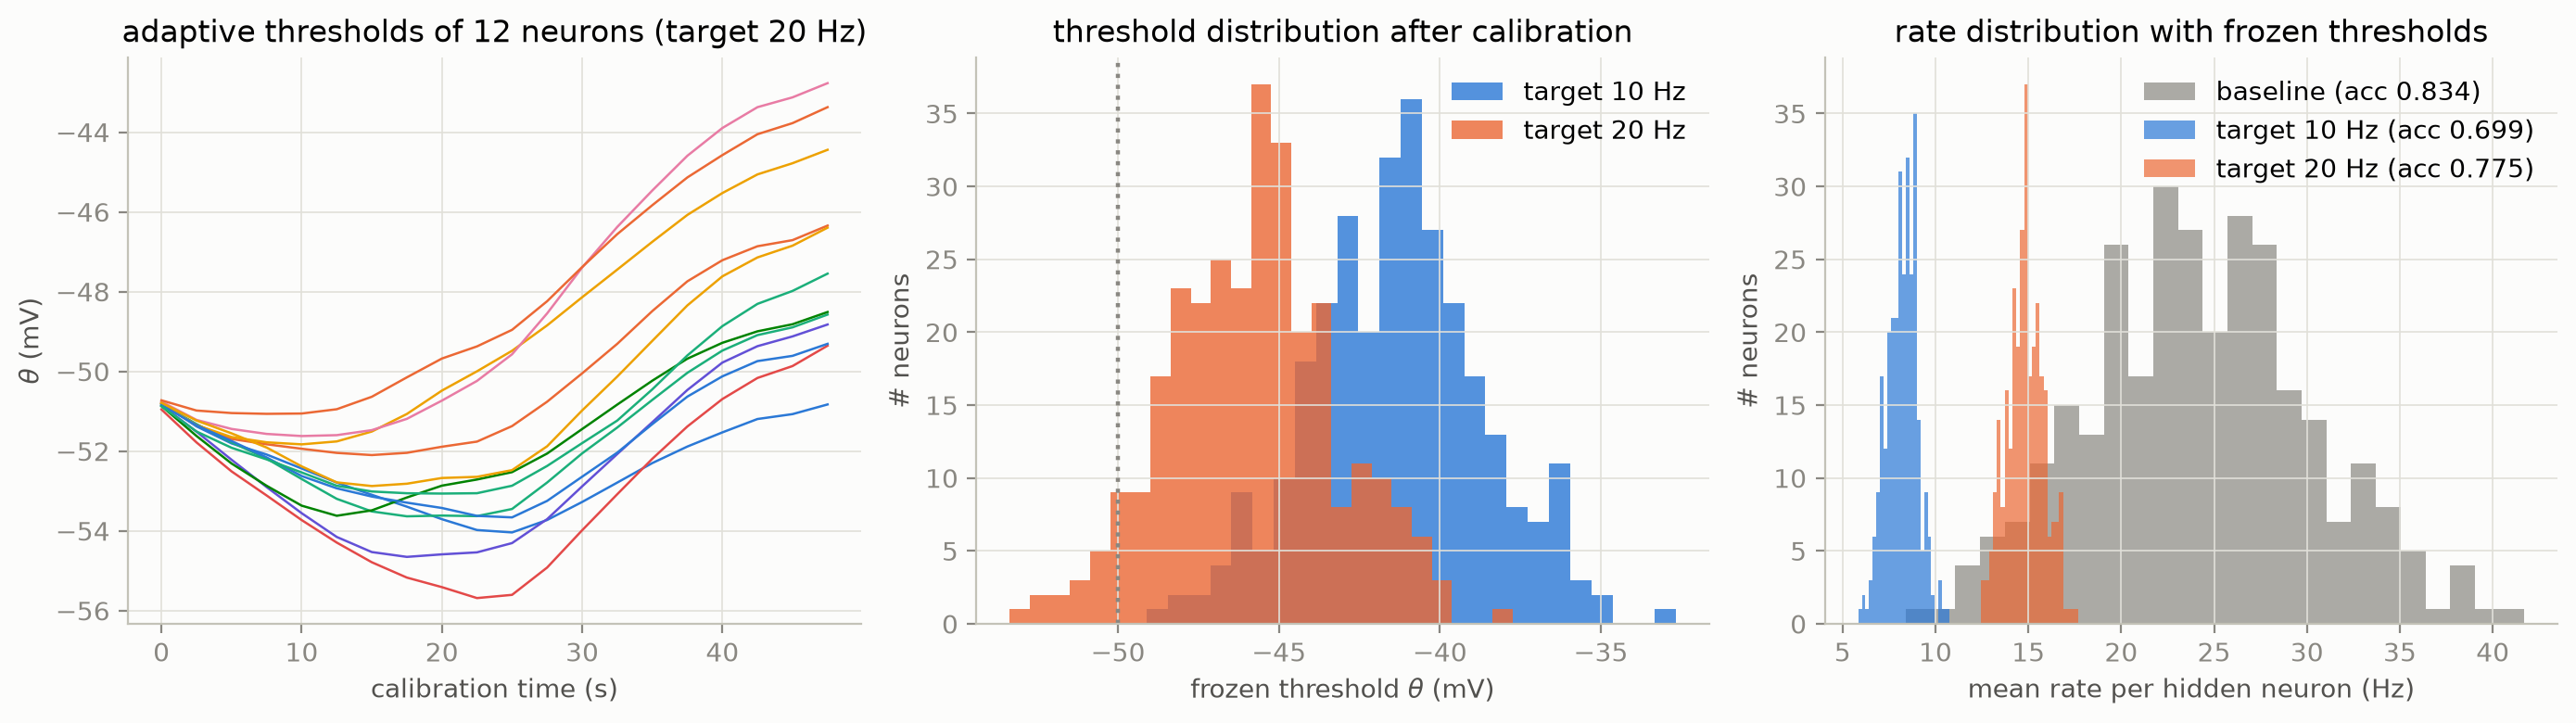
\includegraphics[width=\textwidth]{fig_homeostasis.png}
\caption{Homeostatic threshold regulation. Left: thresholds of 12 neurons during calibration (target 20~Hz). Middle: distribution of the frozen thresholds. Right: per-neuron firing-rate distribution of the baseline and of the two homeostatic networks.}
\label{fig:homeo}
\end{figure}

\begin{table}[h]
\centering
\caption{Homeostatic regulation versus the baseline.}
\label{tab:homeo}
\begin{tabular}{lcccc}
\toprule
Network & Accuracy & Macro-F1 & Rate mean $\pm$ s.d. (Hz) & Spikes/image\\
\midrule
HOMEO\_ROWS
\bottomrule
\end{tabular}
\end{table}

HOMEO\_ANALYSIS

\subsection{Conclusions}
CONCLUSIONS

\end{document}
